\documentclass[a4paper, 11pt, normalem]{report}

\usepackage{../../../LaTeX-Templates/Notes}

\titlecontents{chapter}% <section-type>
    [0pt]% <left>
    {}% <above-code>
    {Lecture \thecontentslabel\quad}% <numbered-entry-format>
    {}% <numberless-entry-format>
    {\dotfill\contentspage}% <filler-page-format>
\titleformat{\chapter}{\fontsize{13}{15}\bfseries\normalfont}{\textbf{Lecture \thechapter}}{1em}{}
\titleformat{\subsection}{\fontsize{10}{15}\bfseries\scshape}{\textbf{Example \thesubsection}}{1em}{}
\setcounter{tocdepth}{4}
% \setcounter{secnumdepth}{1}

\newcommand\p{\partial}

\newcommand\answerbox{%%
    \fbox{\rule{0.8in}{0pt}\rule[-0.5ex]{0pt}{3ex}}}

\newcommand\halfbox{%%
    \fbox{\rule{0.36in}{0pt}\rule[-0.25ex]{0pt}{3ex}}}

\renewcommand{\arraystretch}{1.2}

\title{Foundations of Physics 2B \\ Thermodynamics \vspace{-20pt}}
\author{Dr Peter Swift}
\date{\vspace{-15pt}Michaelmas Term 2017}
\rhead{\hyperlink{page.1}{Go to TOC}}

\begin{document}

\maketitle
\thispagestyle{fancy}

\tableofcontents

\chapter{}
\section{Intro}
This course will frame concepts in concrete maths from last year

Laws:
\begin{itemize}
  \item Zeroth establishes the meaning of temperature
  \item First is a statement of energy conservation [we can only break even]
  \item Second defines entropy -- why things do or do not happen
  \begin{itemize}
    \item[--] Entropy measures energy quality [you can only break even at 0 K]
  \end{itemize}
  \item Third doesn't define thermodynamic property; tells us we can't get to 0 K
\end{itemize}

Thermodynamics developed by engineers wanting to develop machines that turn heat to work \\
Wanted most work for least effort \\
Subject developed had a number of under-ranging consequences \\
When it emerged, atoms were unknown -- considered average properties of bulk material \\
There was no attention paid to what was inside \\
Macroscopic approach to look at 'black box':
\begin{itemize}
  \item[--] This approach is general and difficult to 'see the point' \\
  All good having relationships about heat capacities and expansicities but tells us nothing about the physics
  \item[e.g.] why a material has a certain temperature dependence for its heat capacity
\end{itemize}

Opening the black box gets microscopic picture (atomic) but this can be very detailed ($N_A \approx 6 \times 10^23$) \\
Statistical mechanics instead looks at average properties of all atoms in the thermodynamic limit

\subsection{Counting Molecules -- simpler than recording position and motion  as fewer DoFs}
Lecture theatre has $10^29$ molecules ($3 \times 10^6$ litres of air) \\
A 10GhZ processor can count $10^17$ molecules per year (each cycle counts one) $\approx 3 \times 10^11$ years to count all molecules \\
Thermodynamic limit -- things tend to the average (to infinity)

\subsection{Rains drops hit small and large roof:}
Fluctuations in force smooth out, even through force increasing \\
Consider pressure, $p = \frac{F}{A}$, same in both cases if you consider the average \\
Thermodynamic limit -- $A \to \infty$

\section{Thermo Systems and States}
\begin{tabular}{c|c|c}
     & Extensive -- System Extent & Intensive -- Independent \\
     \hline
     \multirow{2}{7em}{\answerbox} & Volume, V & Temp, T \\
     & Energy, U & Pressure, P \\
     \hline
     \multirow{2}{7em}{\halfbox \halfbox} & $V = V_A = V_B = \frac{V}{2}$ & $T^* = T_A = T_B = T$ \\
     & $U = U_A = U_B = \frac{U}{2}$ & $p^* = p_A = p_B = p$
\end{tabular}

Relate properties by equation of state, $f(p,V,T) = 0$ \\
Most well known as the ideal gas law: $pV = nRT$

\section{Thermal Equilibrium (TE), Heat, and Temperature}
Can prepare sample of gas by suitable treatment to take a range of values of pressure and volume
\begin{equation*}
    p_{1}V_{1} = a > b = p_{2}V_{2} \text{ -- Sample 1 is hotter than Sample 2}
\end{equation*}
Equation of state, $pV = f(T)$

Heat is thermal energy in transit, heat transferred from hot to cold (under its own action) \\
In transit is important -- can't say object contains an amount of heat \\
Addition/subtraction of heat changes temperature \\
If two objects have the same temperature, they're in TE

Heat capacity -- $\Delta Q = mc\Delta T$ \\
More rigorously, a small change, dT, in a substance's temperature, requires the addition/subtraction of a differention and of heat,  $\delta Q$:
\begin{equation*}
    \delta Q = mcdT
\end{equation*}
Capital C: Heat capacity of whole substance \\
Lower c: Specific heat capacity per unit mass/mole \\
$C = mc$

Total heat energy to change temperature, $T_1 \to T_2$:
\begin{equation*}
    \Delta Q = \int_{T_{1}}^{T_{2}} \delta Q = \int_{T_1}^{T_2} mcdT
\end{equation*}
Most changes take place whilst some other property is held constant:
\begin{gather*}
    C_{V} = \Big(\frac{\p Q}{\p T}\Big)_{V};~~ C_{p} = \Big(\frac{\p Q}{\p T}\Big)_{p}
    C_{p} > C_{V}
\end{gather*}
Work is needed to keep at constant pressure -- work is a form of energy so requires more heat energy in to get to the same temperature at constant pressure

\chapter{}
\section{Zeroth Law}
\emph{"If two system are separately in TE with a third system, they must be in TE with each other"}

If heat flows between two systems, they can't spontaneously turn back to initial states. \\
If two objects are at the same temperature, they're in TE \\
This defines the arrow of time

Thermometers have a low heat capacity relative to the object they're measuring

\section{Relevant Maths}
Thermodynamics is concerned with properties that change \\\
Changing one (e.g. temp) will affect others (e.g. pressure) but might hold some more (e.g. volume) constant \\
Always denote what is held constant explicitly
\begin{equation*}
    C_p = \Big(\frac{\p Q}{\p T}\Big)_p \neq \Big(\frac{\p Q}{\p T}\Big)_V = C_V
\end{equation*}

\subsection{}
Kinetic energy in gases: $U = \frac{1}{2}m<v>^2 = \frac{3}{2}Nk_{b}T$ \\
Look at ideal gases for simplification:
\begin{gather*}
    pV = nRT;~~ n = \frac{N}{N_{A}};~~ R = N_{A}k_{b} \\
    U = \frac{3}{2}Nk_{b}T = \frac{3}{2}pV \\
    \Big(\frac{\p U}{\p V}\Big)_T = 0;~~ \Big(\frac{\p U}{\p V}\Big)_p = \frac{3}{2}p
\end{gather*}
Look at First Law:
\begin{gather*}
    dU = T\,ds - p\,dV \\
    \Big(\frac{\p U}{\p V}\Big)_S = -p
\end{gather*}
Now consider the total differential of $z = f(x,\,y)$, $z = Z(x,\,y)$, or $f(x,\,y,\,z) = 0$ \\
This has two independent variables
\begin{equation*}
    dz = \Big(\frac{\p z}{\p x}\Big)_y dx + \Big(\frac{\p z}{\p y}\Big)_x dy
\end{equation*}
\newpage
\begin{wrapfigure}{r}{0.35\textwidth}
    \begin{center}
        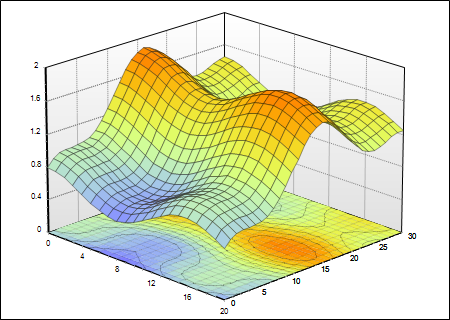
\includegraphics[scale=0.35]{Surface.png}
    \end{center}
\end{wrapfigure}
Infinitesimal change in z resulting from infinitesimal changes in x and y \\
Z represents a surface

Consider an intersection of the surface in the x-z plane at some y

Rather than consider the value of z, we look at the shape at any point of the lines of intersection with planes constant x or y

\subsection{}
For $p = p(V,\,T)$:
\begin{gather*}
    dp = \Big(\frac{\p p}{\p V}\Big)_T dV + \Big(\frac{\p p}{\p T}\Big)_V dT \\
    pV = nRT ~~\implies \\
    \Big(\frac{\p p}{\p V}\Big)_T = -\frac{RT}{V^2};~~ \Big(\frac{\p p}{\p T}\Big)_V = \frac{R}{V} \\
    dp = -\frac{RT}{V^2}dV + \frac{R}{V}dT \\
    dp = \frac{RT}{V}\Big(- \frac{dV}{V} + \frac{dT}{T}\Big)~~ \Big[p = \frac{RT}{V}\Big] \\
    \frac{dp}{p} = - \frac{dV}{V} + \frac{dT}{T} \\
    d(\ln{p}) = -d(\ln{V}) + d(\ln{T})~~ \Big[\frac{d(\ln{x})}{dx} = \frac{1}{x} \Big]
\end{gather*}

\subsubsection{Proof 2.2.2.1}
x, y, and z related via $f(x,\,y,\,z)$
\begin{gather*}
    x = X(y,\,z)~;~ y = Y(x,\,z) \\
    dx = \Big(\frac{\p X}{\p y} \Big)_z dy + \Big(\frac{\p X}{\p z} \Big)_y ~;~ dy = \Big(\frac{\p Y}{\p x} \Big)_z dx + \Big(\frac{\p Y}{\p z} \Big)_x dz \\
    dx = \Big(\frac{\p x}{\p y} \Big)_z \Big(\frac{\p y}{\p x} \Big)_z dx + \Bigg[\Big(\frac{\p x}{\p y} \Big)_z \Big(\frac{\p y}{\p z} \Big)_x + \Big(\frac{\p x}{\p z} \Big)_y \Bigg] dz \\
    dx = M(x,\,y)\,dx + N(x,\,y)\,dz
\end{gather*}
For $M = 1$:
\begin{equation*}
    \Big(\frac{\p x}{\p y} \Big)_z \Big(\frac{\p y}{\p x} \Big)_z = 1 \text{ -- Reciprocal Theorem}
\end{equation*}
For $N = 0$:
\begin{gather*}
    \Big(\frac{\p x}{\p y} \Big)_z \Big(\frac{\p y}{\p z} \Big)_x + \Big(\frac{\p x}{\p z} \Big)_y = 0 ~~ \Bigg[ \times \Big(\frac{\p z}{\p y} \Big)_y \Bigg] \\
    \Big(\frac{\p x}{\p y} \Big)_z \Big(\frac{\p y}{\p z} \Big)_x \Big(\frac{\p z}{\p y} \Big)_y + 1 = 0 \\
    \Big(\frac{\p x}{\p y} \Big)_z \Big(\frac{\p y}{\p z} \Big)_x \Big(\frac{\p z}{\p y} \Big)_y = -1 \text{ -- Reciprocity Theorem (Cyclic)}
\end{gather*}
Well-behaved functions (as above) are exact differentials

For $z = f(x,\,y)$ with two independent variables
\begin{equation*}
    dz = M(x,\,y)\,dx + N(x,\,y)\,dy
\end{equation*}
If exact:
\begin{gather*}
    \Big(\frac{\p M}{\p y} \Big)_x = \Big(\frac{\p N}{\p x} \Big)_y \\
    \frac{\p}{\p y}\Bigg[\Big(\frac{\p M}{\p y} \Big)_x \Bigg]_y = \frac{\p^2 z}{\p x \p y} \equiv \frac{\p}{\p x}\Bigg[\Big(\frac{\p N}{\p x}\Big)_y \Bigg]_x = \frac{\p^2 z}{\p x \p y}
\end{gather*}
For exact functions, the order of the second derivatives doesn't matter. \\
These are \emph{line integrals}.
\begin{equation*}
    I = \int_{1}^{2} dz = \int M(x,\,y)\,dx + \int N(x,\,y)\,dy = Z_2 - Z_1
\end{equation*}
Parts can be integrated independently and the answer doesn't depend on the path \\
These correspond to functions of state in thermodynamics (p, V, T)

If $\frac{\p^2 z}{\p x \p y} \neq \frac{\p^2 z}{\p y \p x}$, this is inexact, and a \emph{point function}. \\
The value of the integral depends on the path (W, Q)

dV - incremental volume change \\
Total volume change from state 1 to 2:
\begin{equation*}
    \int_{1}^{2} dV = V_2 - V_1 = \Delta V
\end{equation*}
If we return to original state, the path is closed:
\begin{equation*}
    \oint dV = 0
\end{equation*}
The work between two states is path dependent:
\begin{equation*}
    W_{1 \to 2} = \int_{1}^{2} \delta W \neq W_2 - W_1
\end{equation*}
\begin{wrapfigure}{l}{0.4\textwidth}
    \begin{center}
        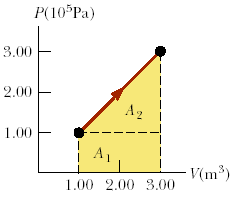
\includegraphics[scale=0.6]{WorkPV.png}
    \end{center}
    \vspace{-120pt}
\end{wrapfigure}

Differential works along the path are added.
\begin{gather*}
\left.\begin{aligned}
       \Delta V_1 &= V_2 - V_1 \\
       \Delta V_2 &= V_2 - V_1
      \end{aligned}
\right\}
    \quad \text{exact dV, path independent} \\
    W_1 \neq W_2 ~ \text{ -- areas are different, so inexact } \delta W
\end{gather*}

\newpage
\subsection{}
\begin{wrapfigure}{r}{0.4\textwidth}
    \begin{center}
        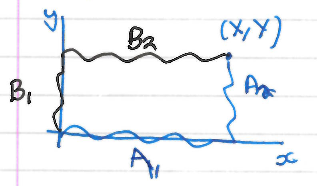
\includegraphics[scale=0.5]{XYCord.png}
    \end{center}
\end{wrapfigure}
Consider $\delta F = x\,dx + x\,dy$ (inexact) with two paths for $(0,\,0) \to (X,\,Y)$

Path A: $(0,\,0) \to (X,\,0) \to (X,\,Y)$ \\
Path B: $(0,\,0) \to (0,\,Y) \to (X,\,Y)$
\begin{flalign*}
    A &=
    \begin{cases}
        A_1 & \int_{A_1} \delta F = \int_{0}^{X} x\,dx + \cancel{\int_{0}^{0} x\,dy}^{dy = 0} = \frac{X^2}{2} \\
        +   & \\
        A_2 & \int_{A_2} \delta F = \cancel{\int_{X}^{X} X\,dx}^{dx = 0} + \int_{0}^{Y} X\,dy = [Xy]_{0}^{Y} = XY
    \end{cases}
    \\\\
    \int_{A} &\delta F = \int_{A_1} + \int_{A_2} = \frac{X^2}{2} + XY ~~;~~ \int_{B} \delta F = \frac{X^2}{2}
\end{flalign*}

































\end{document}
